\section{Level Editor}\label{ch:leveleditor}
\subsection{Manual Levelgenerator}
\subsubsection{Preexisting Levelgenerator}
As a base we used an already existing leveleditor\footnote{http://www.battlefieldsingleplayer.com/apachethunder/angrybirds/} which works by selecting from a number of objects and positioning them with the keyboard.
By pressing save the level is downloaded as Lua file. 
\subsubsection{Parser for Format Change}
We wrote a parser that takes all levels from the levelsToParse folder and converts them to json files.
If 'Bird' was in the original level format (Lua file) we concatenated 'bird\_' and the number of the bird otherwise we the key was 'block\_' and the number of the block.
The position in the original format and the position in the game we needed was not the same so we multiplied it with 0.91 which differs if you start to zoom into the levelgenerator and position the blocks closer to each other. Then the 0.91 can be removed. The parser also adds 52 to the x value of the blocks and put all birds behind the slingshot.
The blocks in the levelgenerator can be turned in either way and result in different angles depending if they were turned to the right (positive radian) or to the left (negative radian). We converted them to positive degree values.
The names of the blocks, pigs and the birds differ as well in the two formats, we solved this with a dictionary where the names from the lua file are the key and the names of our version are the values. The parser then chooses the value for the found key from the Lua file to get the name of the structure, bird or pig. We convert the longest breakable structure block to terrain as this structure block does not exist in the version of the game that we use.
The parser also removes the preexisting blocks and the pig of the editor. We added code to remove the birds aswell but they are currently commented out so this can be adapted if the user wishs to remove the birds, too.
After converting the content which is described above the prefile.json which contains the additional necessary json code is added as well as the number of blocks and birds.
The place where the converted level is saved is parsedLevels per default. This can be changed to the slingshot folder of the game in the parser. 

\subsubsection{How to Use the Manual Levelgenerator}
\begin{enumerate}
	\item \textbf{Open the Editor Locally}
	
	Go to the directory `levelGenerator/manualLevelGeneratorJS/` and open the index.html in your webbrowser.
	\item \textbf{Create the Level}
	
	Create the level you want, you can put the birds where you want as they will moved to the correct position anyways. You can use \textbf{all kinds of birds and pigs} in the game. The other things you can use are limited to \textbf{all blocks of stone, ice, wood, static breakable structure and terrain}. The latest two look same in the editor but can be differentiated through the code on the top of the page.
	You can position the blocks and pigs from the very left side of the window to the very right side. It is better to not zoom in, which is possible with the up and down arrow key, as the factor of 0.91 would not fit anymore and the very left side could not be used to place objects anymore. The factor with zooming in could be 1 for example. This is the case because then the objects fit closer together so if you put two items right next to each other they would be closer together than without zooming in. When the factor is not adapted in this case, the objects are too close together and structures can collapse.
	Most of the hints for editing are already given in the editor itself. To delete objects you only have to press the delete key.
	
	\item \textbf{Save Level} Click at save and save the level to a folder.
	
	\item \textbf{Adapt Paths} Open the Parser.py and adapt all paths to your personal structure (optional: only if not already done before).

	\item \textbf{Run Parser} Run the Parser.py with python3

	\item \textbf{Copy File} If you did not change the structure of the output-file to the json directory where you run your game \footnote{if you run the game in slingshot this would be in `cors/fowl/json/`} copy the file now in this directory (optional: only if not changed before)

	\item \textbf{Run Game} Run Angrybirds (now you should see the new level you just created, if this is not the case check if your machine cached the levels)
	
\end{enumerate}

\subsection{Random Levelgenerator}
\label{Random LevelGenerator}
\subsubsection{General}
	The random levelgenerator can create different kinds of levels. The number of the levels of the different types can be changed in the main class:
	\begin{description}
		\item[Main](\class{levelGenerator.main})\\
			The main method calls the createLevel methods with the number of levels that should be generated. 
		\item[LevelCreator](\class{levelGenerator.LevelCreator})\\
			This class calls the create method of the BasicLevel with the parameter and the type of level that was requested. In addition to the level types below it can generate a simple level where the Basic Level is called with no structure to add.
		\item[BasicLevel](\class{levelGenerator.LevelCreator})\\
			Adds the basic things the LevelN-M.json file needs to actually work as level like f.e. the camera.
			It also adds as many randomized blocks, pigs, terrainblocks as the method was called with as well as the structure and the red birds.
			This class can also receive a list with all positions of the blocks of the structure and put the blocks around it. This feature does not work for all kinds of levels yet. 
	\end{description}
\subsubsection{Structure Levels}
\begin{description}
	\item[DominoLevel](\class{levelGenerator.DominoStructure})\\
		The level contains three vertical large blocks that are positioned on the ground and their distance and material is picked randomly. The distance and the material is for all blocks the same. For this level the pigs and a chosen amount of random blocks are positioned randomly by the LevelCreator class.
		\begin{figure}[tbh!]
			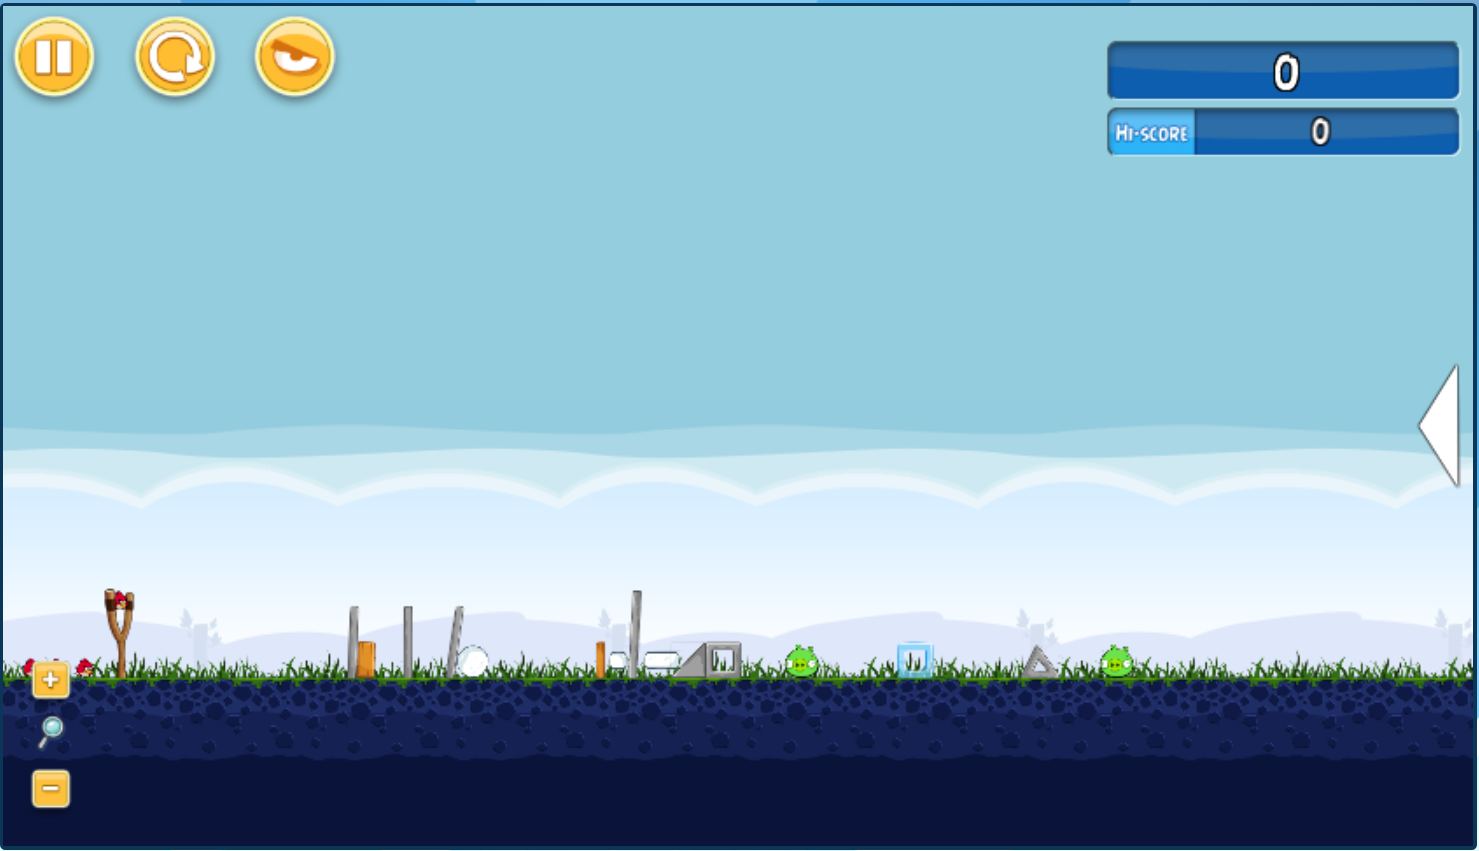
\includegraphics[width=0.5\textwidth]{img/DominoLevel.png}
			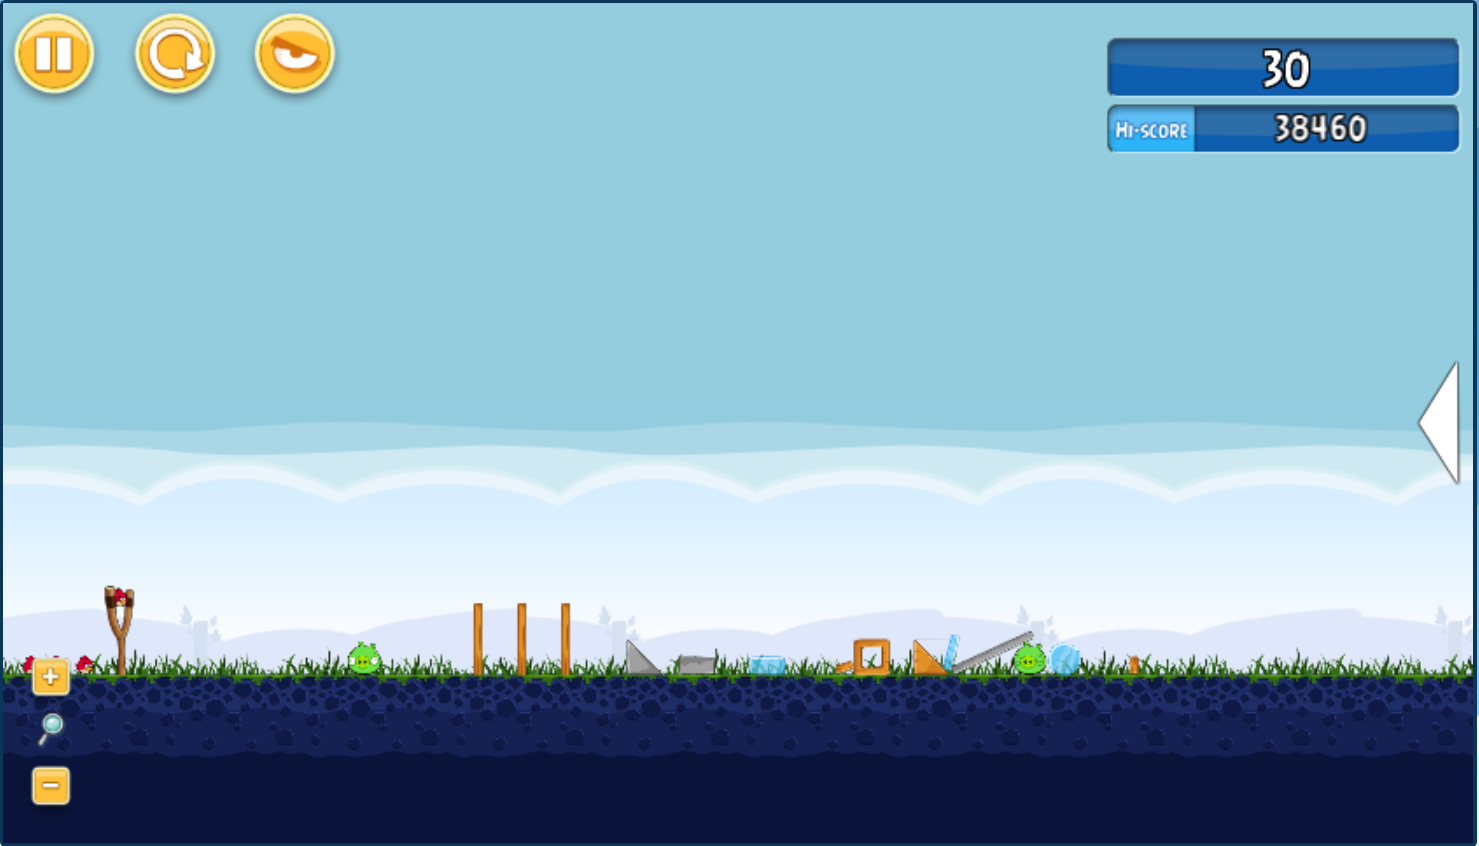
\includegraphics[width=0.5\textwidth]{img/DominoLevel2.png}
			\caption{Two examples of DominoLevels}
		\end{figure}
	\item[HouseLevel](\class{levelGenerator.HouseStructure})\\
		In this level houses build out of three long blocks are created. The structure can randomly be either on the ground or on a static block in the air. Where the structure is and what material it is build of depends on the random values. The material of all blocks is the same and only large blocks can be chosen. The first level of the structure can have up to three houses and can have a second level with one house less. The pigs positioned in the level are all the same but picked randomly and positioned in each house of the first level of the structure.
		\begin{figure}[tbh!]
		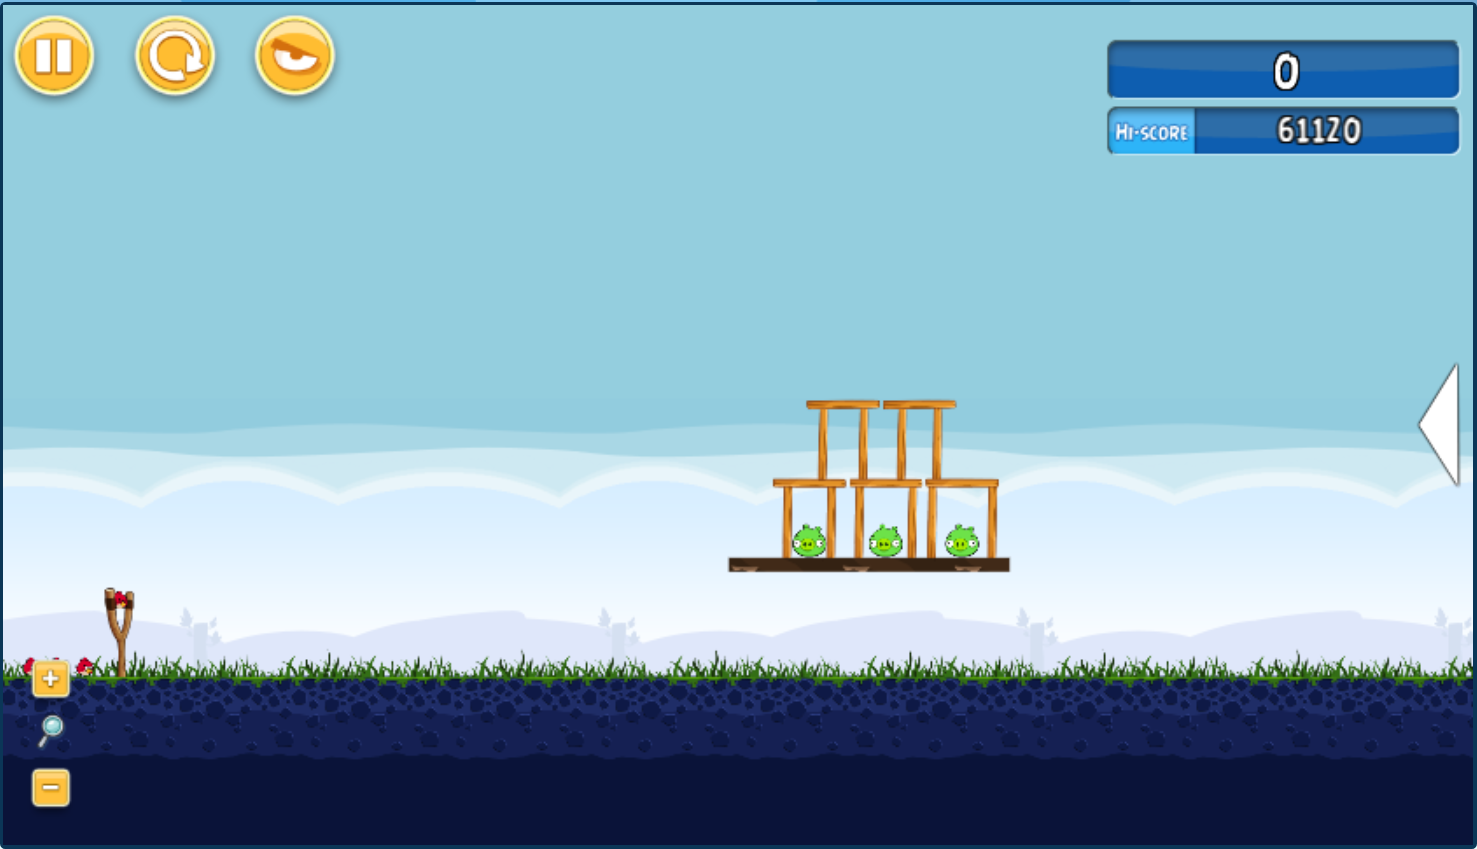
\includegraphics[width=0.5\textwidth]{img/HouseLevel.png}
		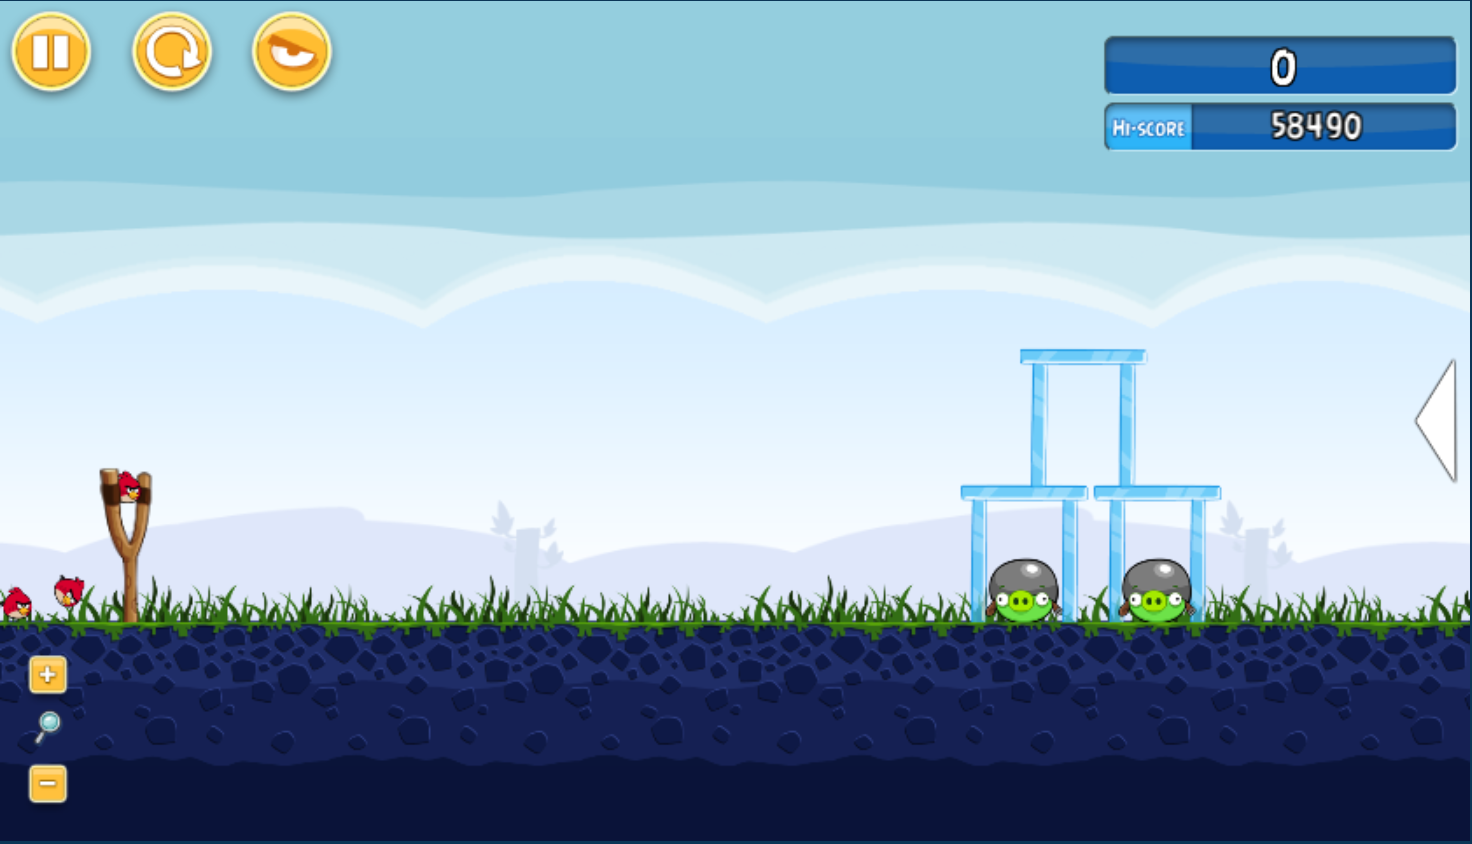
\includegraphics[width=0.5\textwidth]{img/HouseLevel2.png}
		\caption{Two examples of HouseLevels}
		\end{figure}
	\item[FunnelLevel](\class{levelGenerator.FunnelStructure})\\
		For this kind of level a static block is positioned horizontally above the ground so a bird still fits below. At the end of this funnel there is a pig. Random blocks can be positioned all over the level by the LevelCreator class.
		\begin{figure}[tbh!]
			\centering
			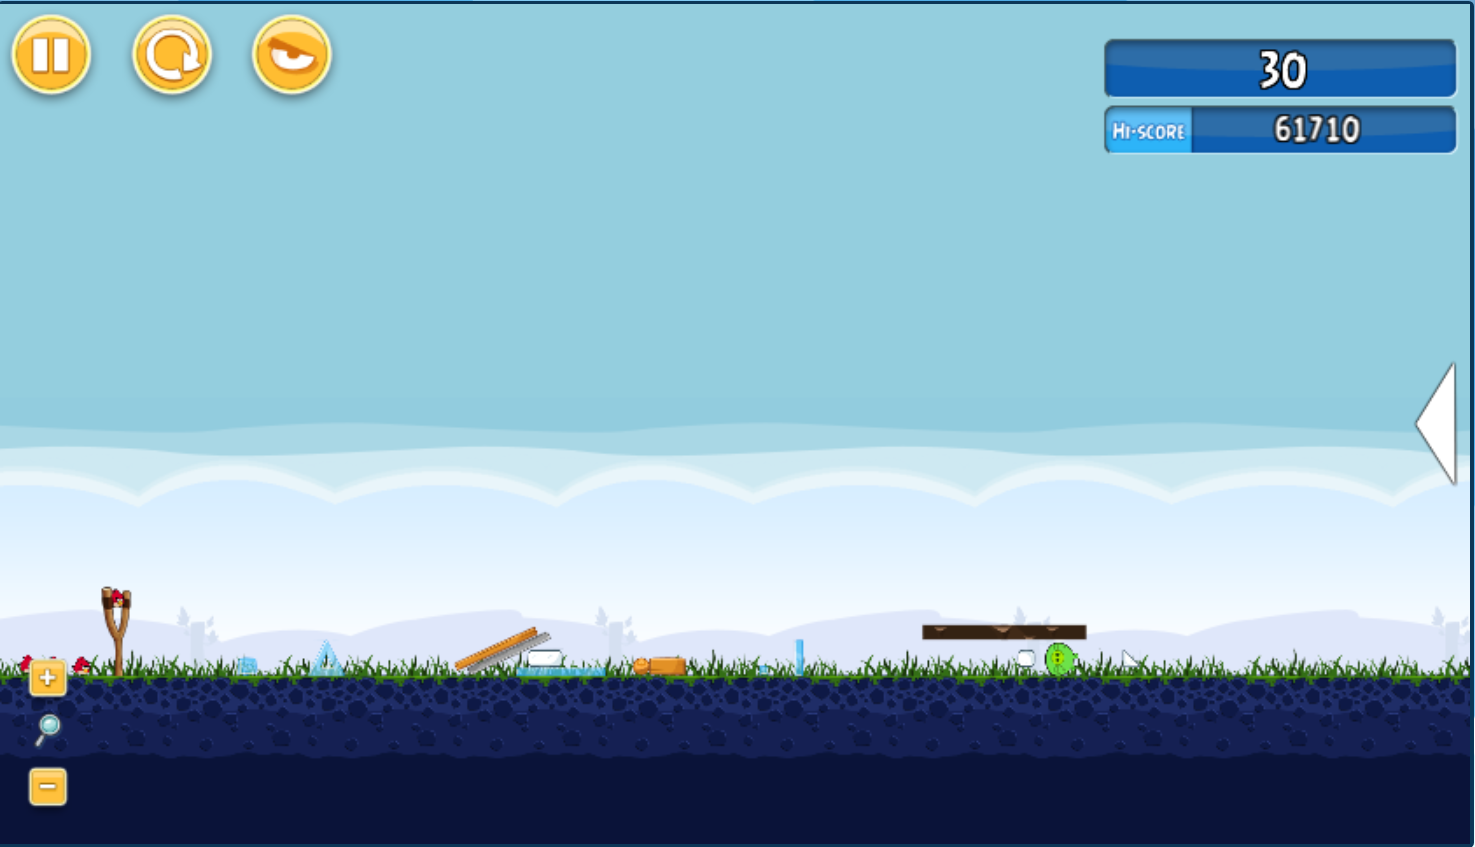
\includegraphics[width=0.5\textwidth]{img/FunnelLevel.png}
			\caption{An example of a FunnelLevel}
		\end{figure}
		\end{description}
\subsubsection{How to Use the Random Levelgenerator}
	\begin{enumerate}
		\item \textbf{Select Levels} Open the Main class and comment/uncomment the calling of the create*-functions in the main method according to the type of levels you want to create. Change the parameter of those method calls to the number of levels you want to create of this type.
		\item \textbf{Run Generator} Run main.java
		\item \textbf{Copy File} Copy the levels to the directory where you want to play the game (json directory), make sure you use only levels of one type at the time or rename them properly (Level1-\textit{1 to 21}.json)\footnote{for example Level1-4.json}. The first number is the page and the second is the level of the page.
		\item \textbf{Run Game} Run Angrybirds
	\end{enumerate}
\subsection{Transformation Values for Editing .json Level Files}

Assuming the x-value for a block in the LevelN-M.json is called \textit{json.x}, and the x-value of the MBR-vision-module is called \textit{mbr.x}, the formula for transforming json.x to mbr.x is: 
\[mbr.x = json.x * 5 + 14\]

Remember that mbr.x (and mbr.y) marks the x-value (and y-value) of the \textit{upper left corner} of the block. The RealShape vision module however returns the \textit{center-values} of each block. 

With the y-values, it is a bit more difficult, since there might be blocks underneath the block that \textit{lower} mbr.y. The baseline (ground line of the level) in the vision-module is 385. Each block-y-value (let that be json.y, e.g. 4 on a vertically aligned WOOD\_BLOCK\_4X1) \textbf{lowers the baseline by 5}, so, the higher the block is, the lower the number gets. A vertically aligned WOOD\_BLOCK\_10X1 has a mbr.y of 335 (`385 - 5 * json.y = mbr.y`), while a vertically aligned WOOD\_BLOCK\_4X1 has a mbr.y of 365.